% Required packages in the main document:
%   \usepackage{graphicx}
%   \usepackage{subcaption}
%   \usepackage{booktabs}
% Figures are expected in ./figures/ relative to the main .tex file.

\section{Weather dataset overview}
\label{sec:data}

The data I'm working with is the \emph{Minute Weather} dataset from Kaggle, originally recorded by a weather station in the HPWREN network around San Diego. It's big: about 1.59 million rows, one row per minute, spanning three years (from 2011-09-10 to 2014-09-10). Each row has a timestamp plus eleven numeric sensor readings --- temperature, relative humidity, air pressure, three wind speeds (min, average, max), the three matching wind directions, rain accumulation, and rain duration. There's also a \texttt{rowID} column which is just the row index, so I ignore it in what follows.

A quick sanity check on the data: missingness is basically not a problem. All six wind columns have 433 missing minutes (0.027\,\%) and the two rain columns have exactly one missing row each. The other variables have no gaps at all. The data does skip some whole days though --- only 1{,}081 out of the 1{,}097 possible calendar days actually show up in the file, so a few days' worth of minutes are simply not there. That's something to watch out for if I want to compute monthly totals later.

One thing about the pressure values stood out right away: the mean is about 917\,mbar, not 1013. That's because the station is clearly at elevation (somewhere around 900\,m / 3{,}000\,ft above sea level). Once I realized that, the rest of the numbers in Table~\ref{tab:summary} made sense: mean temperature 61.9\,$^{\circ}$F, humidity 47.6\,\%, and wind speeds that mostly hang out near 2--3 with occasional gusts up to 36. Rain is the odd one out. 99.4\,\% of the minutes have zero rain accumulation, and 924 out of the 1{,}081 recorded days saw \emph{no} rain at all. So this is basically a dry, semi-arid site.

\begin{table}[h]
    \centering
    \small
    \caption{Summary statistics for the main numeric variables. Wind speeds and rain accumulation are in the native sensor units (the Kaggle page doesn't specify them precisely; rain duration is in seconds). \(N\) differs slightly across rows because of the small amount of missingness mentioned above.}
    \label{tab:summary}
    \begin{tabular}{lrrrrrrrr}
        \toprule
        Variable & $N$ & Mean & SD & Min & Q1 & Median & Q3 & Max \\
        \midrule
        Air temperature ($^{\circ}$F) & 1{,}587{,}257 & 61.85  & 11.83 & 31.64  & 52.70  & 62.24  & 70.88  & 99.50 \\
        Relative humidity (\%)        & 1{,}587{,}257 & 47.61  & 26.21 & 0.70   & 24.70  & 44.70  & 68.00  & 93.00 \\
        Air pressure (mbar)           & 1{,}587{,}257 & 916.83 & 3.05  & 905.00 & 914.80 & 916.70 & 918.70 & 929.50 \\
        Avg wind speed                & 1{,}586{,}824 & 2.77   & 2.06  & 0.00   & 1.30   & 2.20   & 3.80   & 32.30 \\
        Max wind speed                & 1{,}586{,}824 & 3.40   & 2.42  & 0.10   & 1.60   & 2.70   & 4.60   & 36.00 \\
        Min wind speed                & 1{,}586{,}824 & 2.13   & 1.75  & 0.00   & 0.80   & 1.60   & 3.00   & 32.00 \\
        Rain accumulation             & 1{,}587{,}256 & 0.00   & 0.96  & 0.00   & 0.00   & 0.00   & 0.00   & 655.01 \\
        Rain duration (s)             & 1{,}587{,}256 & 0.54   & 81.15 & 0.00   & 0.00   & 0.00   & 0.00   & 63{,}305 \\
        \bottomrule
    \end{tabular}
\end{table}

\begin{figure}[h]
    \centering
    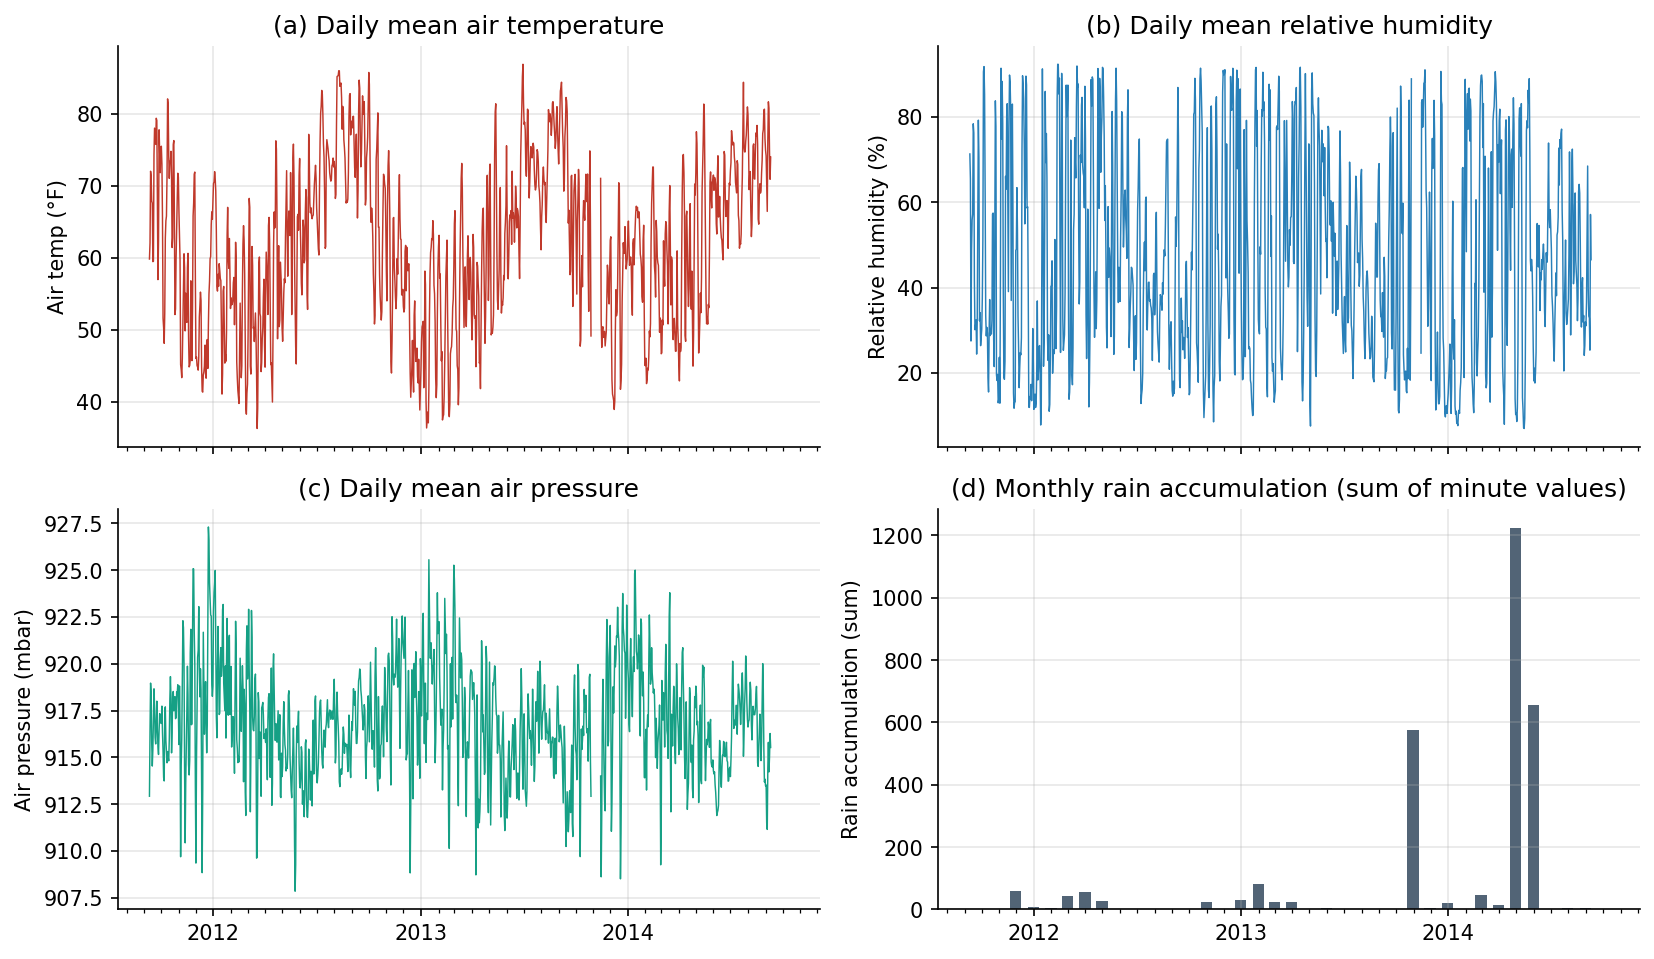
\includegraphics[width=\linewidth]{figures/fig1_timeseries.png}
    \caption{Daily mean values over the three-year record for temperature (a), relative humidity (b), and pressure (c), plus monthly-summed rain accumulation (d). The annual cycle in temperature is obvious; rain is sparse and clumpy.}
    \label{fig:ts}
\end{figure}

Figure~\ref{fig:ts} gives the big-picture view. The temperature panel shows a clean annual cycle with summer peaks around 85\,$^{\circ}$F and winter lows near 40\,$^{\circ}$F --- three years, three cycles, all lining up nicely. The humidity panel looks much noisier day-to-day, but if I squint I can still see the tendency for higher humidity in winter months. Pressure hovers in a narrow 912--928\,mbar band with no strong seasonal trend, which is about what I'd expect at this latitude. The rain panel is the most surprising one: 2012 was almost entirely rainless at this station, while 2014 has two very large monthly totals around spring/early summer. That's odd, since San Diego normally gets its rain in winter, so I want to come back to those big bars once I look at the rain data event-by-event.

\begin{figure}[h]
    \centering
    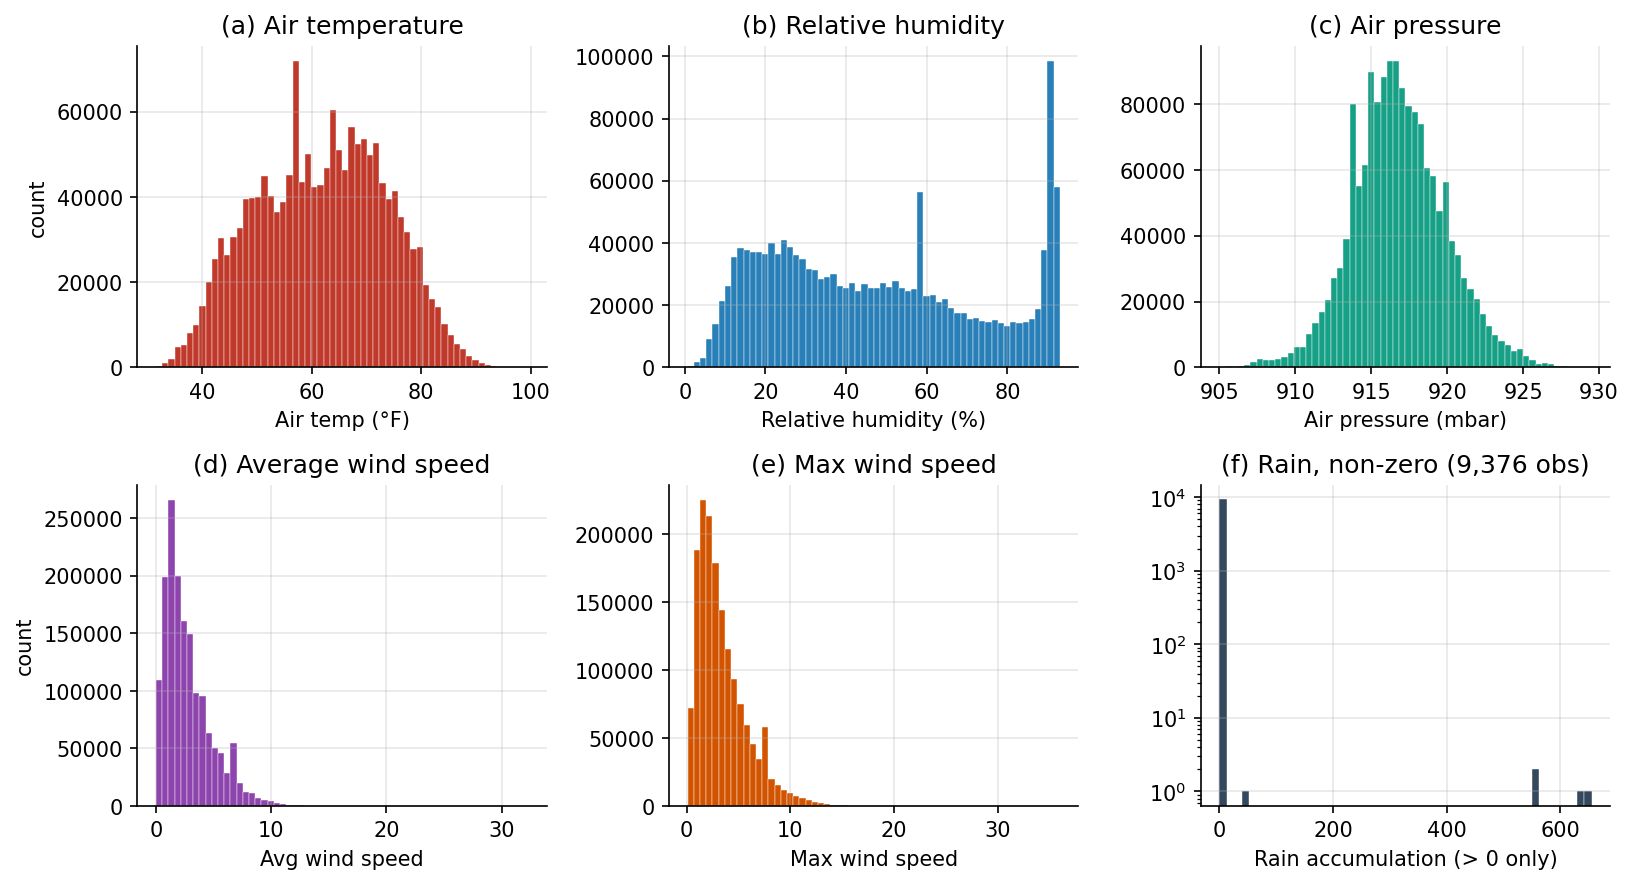
\includegraphics[width=\linewidth]{figures/fig2_distributions.png}
    \caption{Marginal distributions of the main sensor variables. Note the clipping near 90\,\% for humidity in (b) and the log scale on the rain panel (f), which only shows the non-zero minutes.}
    \label{fig:dist}
\end{figure}

The marginal distributions in Figure~\ref{fig:dist} give me a better feel for each variable on its own. Temperature (a) is roughly bell-shaped with a handful of suspicious spikes at specific integer-looking values, which I read as sensor rounding. Humidity (b) is the most interesting shape: it's kind of bimodal, but more importantly there's an \emph{obvious} pile-up at the right edge around 90\,\%. The sensor is almost certainly capped there, so I should be careful about interpreting the upper tail as real moisture variation. Pressure (c) is the best-behaved variable in the whole dataset --- a clean Gaussian centered near 917\,mbar. Wind speeds, both average (d) and max (e), are strongly right-skewed with a mode near 1; calm conditions dominate, and the long tail only occasionally reaches into the 30s. Panel (f) shows only the 9{,}376 non-zero rain minutes and I had to put the $y$-axis on a log scale because most of those values are tiny and only a few events are extreme.

\begin{figure}[h]
    \centering
    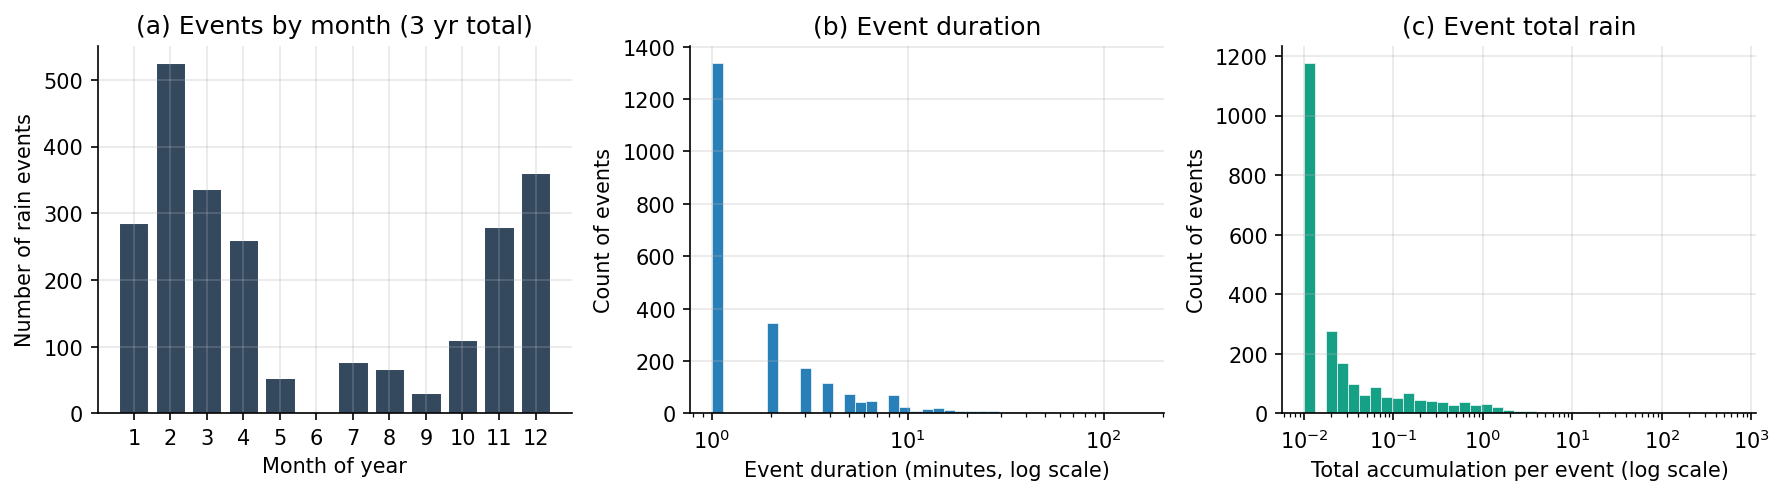
\includegraphics[width=\linewidth]{figures/fig5_rain_events.png}
    \caption{Rain events, defined here as maximal runs of consecutive minutes with \texttt{rain\_accumulation} $> 0$. (a) number of events starting in each calendar month, summed over all three years; (b) distribution of event duration in minutes; (c) total accumulation per event. Both histograms use log-scaled $x$-axes because of the heavy right tails.}
    \label{fig:rain}
\end{figure}

The plain histograms in Figure~\ref{fig:dist}(f) are misleading for rain because of the zero-inflation, so in Figure~\ref{fig:rain} I regrouped the minutes into rain \emph{events}. That gives 2{,}383 events across three years. Panel~(a) shows the strong seasonality the daily time series was hiding: nearly all rain falls between October and April, with February as the clear winter peak, and May--September almost totally dry. That is exactly what a Mediterranean/coastal-California climate looks like. Panel~(b) is the finding I wasn't expecting: the median event duration is just one minute, and 56\,\% of events last exactly one minute. Those are almost certainly drizzle or sensor blips, not storms. The long tail does reach up to about 150 minutes for the biggest events. Panel~(c) confirms that most events are tiny ($<0.1$ accumulation units), but there are a few large ones, and in fact one single event with a total of 655 is what drives the ``spring 2014'' bar in Figure~\ref{fig:ts}(d). So that big bar is really one event, not a rainy month. Whether it's a genuine cloudburst or a sensor artifact I can't tell from this data alone, but it's clearly a single outlier that I should flag before using the rain columns downstream.

\begin{figure}[h]
    \centering
    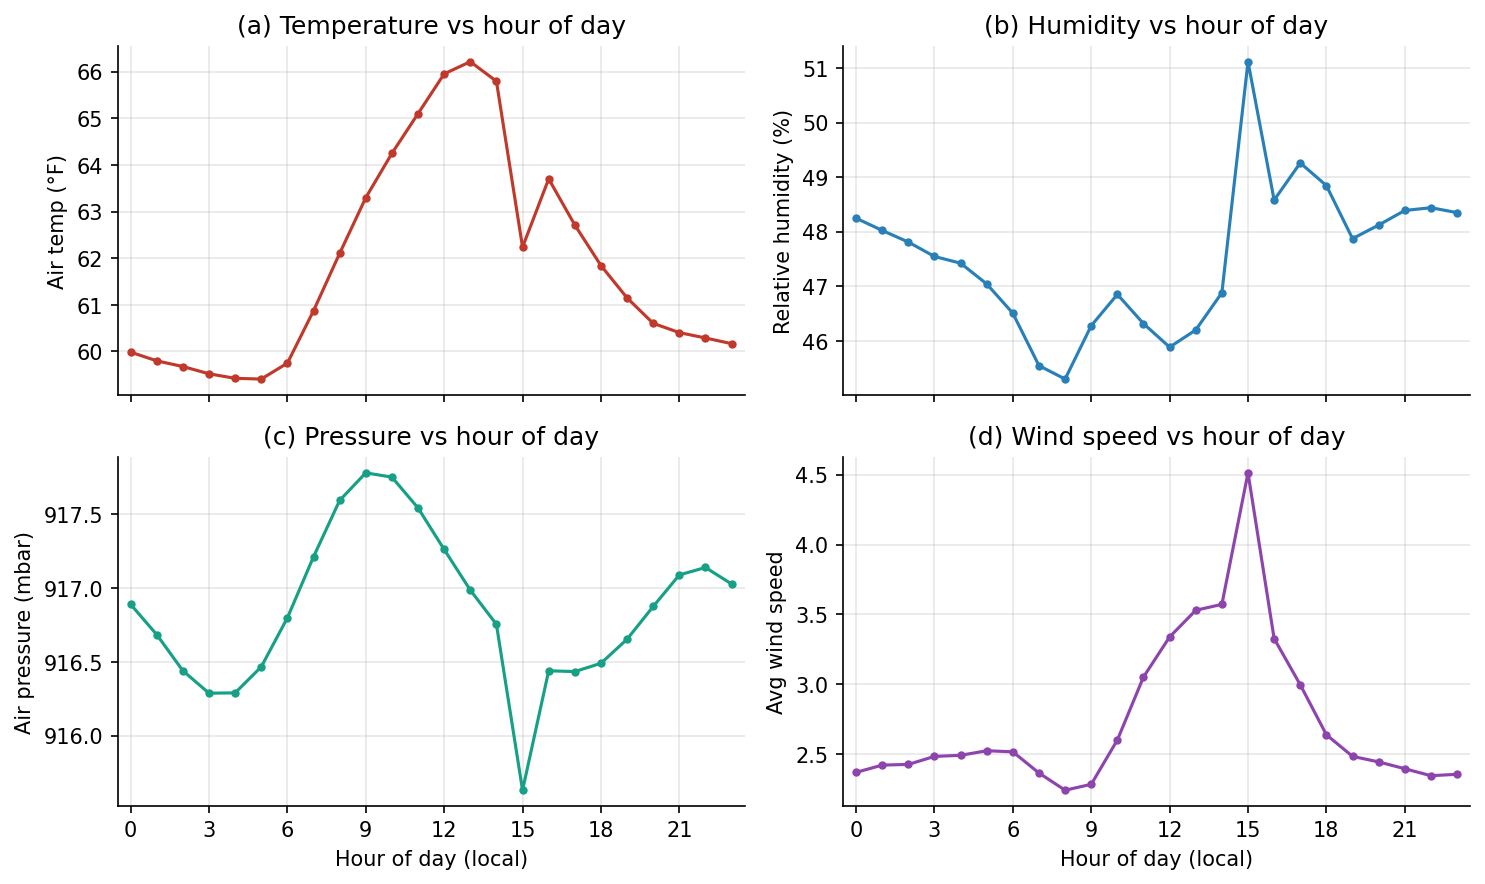
\includegraphics[width=\linewidth]{figures/fig3_diurnal.png}
    \caption{Mean values by hour of day, averaged over the full three-year record. The sharp changes around 15:00 local time are discussed in the text.}
    \label{fig:diurnal}
\end{figure}

Averaging each variable by hour of day (Figure~\ref{fig:diurnal}) tells a cleaner story than the raw time series did. Temperature peaks in the early afternoon around 66\,$^{\circ}$F and bottoms out just before sunrise at 59\,$^{\circ}$F. Humidity does the expected opposite --- low when it's hot, higher at night. What I didn't expect was the obvious ``3\,pm event'' that shows up in all four panels: between 14:00 and 15:00 the temperature drops by almost 4\,$^{\circ}$F, humidity jumps, pressure drops, and wind speed spikes from about 2.5 to 4.5. That has to be the afternoon onshore / thermally-driven breeze kicking in, which pulls in cooler, moister air. Panel~(c) also shows the well-known semi-diurnal pressure oscillation --- two peaks and two troughs per day --- and it's kind of satisfying to see that textbook atmospheric pattern falling out of averaged minute data.

\begin{figure}[h]
    \centering
    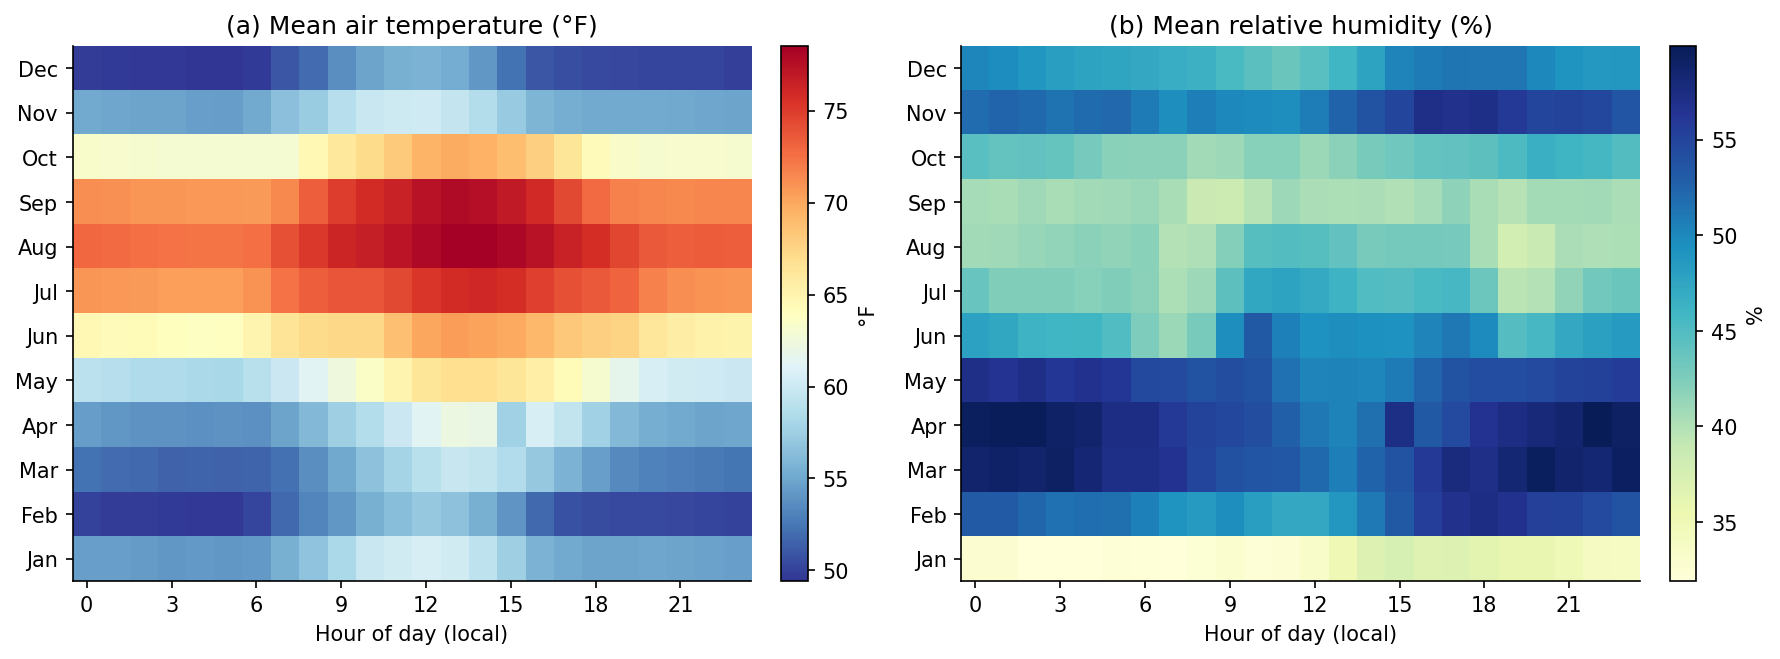
\includegraphics[width=\linewidth]{figures/fig6_month_hour_heatmap.png}
    \caption{Mean temperature (a) and mean relative humidity (b) by month of year ($y$-axis) and hour of day ($x$-axis). Values are averaged across all three years of the record.}
    \label{fig:mh}
\end{figure}

The plain diurnal plot collapses across seasons, so it hides a lot of structure. Figure~\ref{fig:mh} shows the same hourly means but stratified by month. The temperature heatmap (a) has a textbook bullseye: hottest in July--September around 12--15:00, coldest in December early mornings, and the day-to-night amplitude is clearly larger in summer than in winter. The humidity heatmap (b) is more interesting. Spring (March--May) is the most humid band, both day and night. Summer is less humid overall, and the afternoon dry dip that I flagged in Figure~\ref{fig:diurnal}(b) is visible as the lighter vertical stripe around 12--16:00. But the strangest row is January: humidity is the lowest \emph{all day long}, even lower than summer afternoons. I didn't expect winter to be the driest season at this station, but it lines up with the secondary NE peak in the wind rose (Figure~\ref{fig:corr_wind}): Santa-Ana-like offshore winds, which blow very dry desert air toward the coast, happen mostly in winter.

\begin{figure}[h]
    \centering
    \begin{subfigure}{0.54\linewidth}
        \centering
        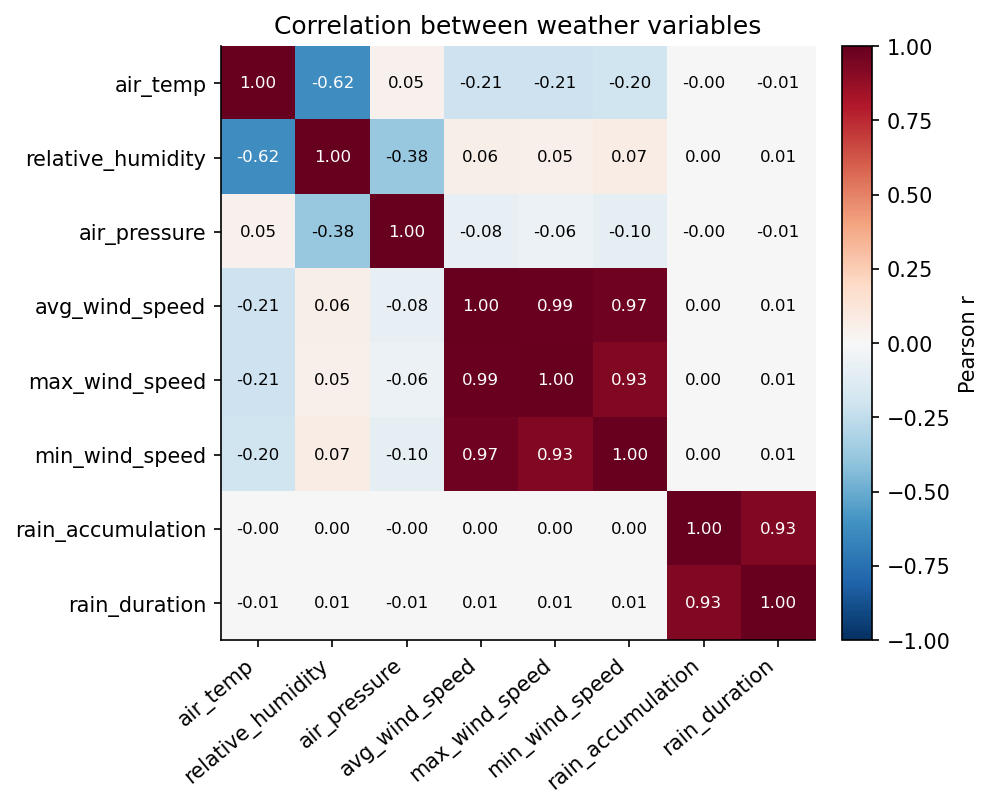
\includegraphics[width=\linewidth]{figures/fig4a_correlation.png}
        \caption{Pearson correlations between the numeric variables.}
        \label{fig:corr}
    \end{subfigure}
    \hfill
    \begin{subfigure}{0.44\linewidth}
        \centering
        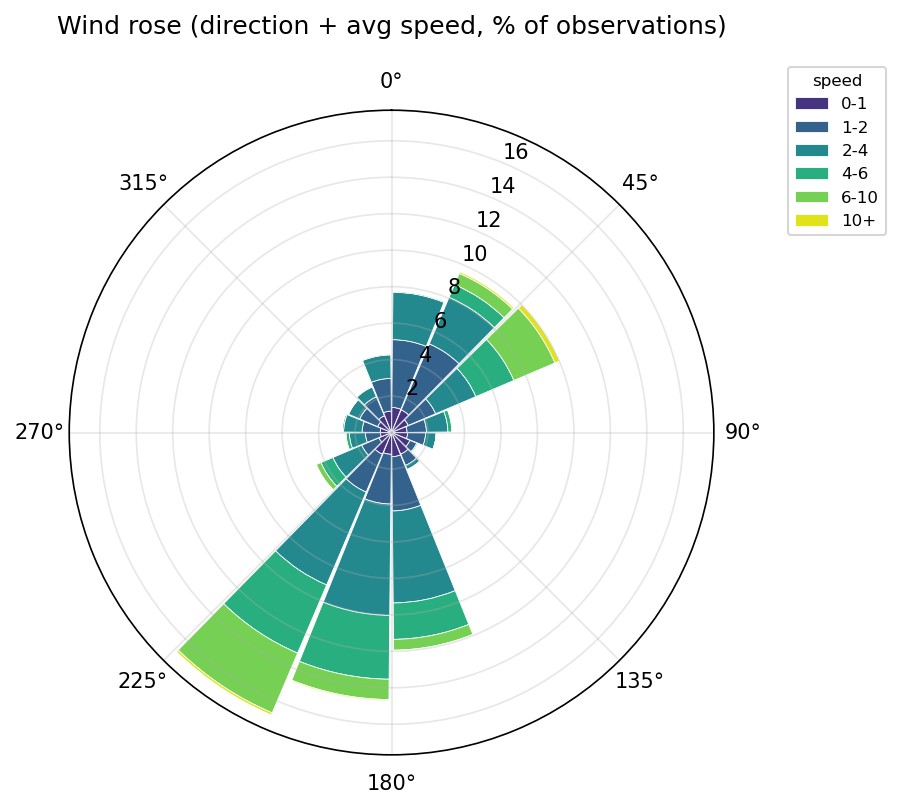
\includegraphics[width=\linewidth]{figures/fig4b_windrose.png}
        \caption{Wind rose: percent of observations binned by direction and average wind speed (brighter colors = faster).}
        \label{fig:wind}
    \end{subfigure}
    \caption{Pairwise relationships between the variables (a) and prevailing wind directions at the station (b).}
    \label{fig:corr_wind}
\end{figure}

Finally, Figure~\ref{fig:corr_wind} summarizes the joint structure. The heatmap on the left (Fig.~\ref{fig:corr}) shows a strong negative temperature--humidity correlation ($r = -0.62$), which is just the usual behavior of relative humidity. Pressure has a moderate negative relationship with humidity ($r = -0.38$) and basically none with temperature. The three wind-speed variables are effectively the same variable pairwise ($r$ between 0.93 and 0.99), so in any downstream model I'll just pick one and drop the other two. Rain accumulation and rain duration are tightly linked as well ($r = 0.93$), which makes sense. Interestingly, rain is essentially uncorrelated with everything else at the minute level, but I think that's mostly a zero-inflation artifact: the 99\,\% of minutes that are dry drown out any real signal, and any real connection between rain and the other variables would show up only once I aggregate up to events or days. The wind rose on the right (Fig.~\ref{fig:wind}) is more informative than I expected. The winds are very far from isotropic: most of the stronger flow comes out of the southwest (roughly 200--225$^{\circ}$), with a smaller but clear secondary peak from the northeast (around 30--50$^{\circ}$), and almost nothing from the east or due north. That bimodal pattern is consistent with a station sitting in complex terrain, where prevailing onshore flow from the Pacific is occasionally interrupted by offshore (Santa-Ana-like) winds coming from the opposite direction, and it's the same NE mode I used above to explain the dry-January row in Figure~\ref{fig:mh}. Practically, this tells me that \texttt{avg\_wind\_direction} won't behave as a well-behaved continuous variable, and if I want to use it later I should probably encode it as $(\sin\theta, \cos\theta)$ or as a categorical variable rather than treating 359$^{\circ}$ as far from 0$^{\circ}$.
